\documentclass[conference,10pt]{IEEEtran}

\usepackage[T1]{fontenc}
\usepackage[utf8]{inputenc}
\usepackage{graphicx}
\usepackage{booktabs}
\usepackage{amsmath,amssymb}
\usepackage{url}

\graphicspath{{../figures/}}

\begin{document}

\title{Comparing Simple Recurrent Neural Networks\\
for Univariate Time Series Forecasting}

\author{\IEEEauthorblockN{Aidan Cohen}
\IEEEauthorblockA{Student number: 27187950}}

\maketitle

\begin{abstract}
Simple recurrent neural networks differ in the values fed back to the
hidden layer.
The study compared three simple recurrent architectures on
one-step-ahead forecasts of five univariate series.
The Elman network feeds back the hidden layer.
The Jordan network feeds back the output.
The multi-recurrent network feeds back both through decaying memory
banks.
The series ranged from a deterministic chaotic system to a stock index
close to a random walk.
The Theil U statistic measured accuracy relative to persistence on
held-out test folds.
Nonparametric tests compared 25 trained networks per architecture on
each series.
The Jordan network was significantly less accurate than both other
architectures on every series except the stock index.
The relative gap between the architectures shrank as the predictability
of the series fell.
The multi-recurrent network gained at most 0.004 in the Theil U
statistic over the Elman network at about four times the weights.
A sensitivity analysis showed the influence of past observations on the
Jordan network fading exponentially with the lag.
Direct access to the delay of the chaotic series reduced the Theil U
statistic of the Jordan network from 0.240 to 0.073.
\end{abstract}

% ======================================================================
\section{Introduction}
\label{sec:introduction}
A time series forecast estimates the next observation of a series from
earlier observations.
The model that produces the forecast therefore needs a memory of the
recent history of the series.
Recurrent neural networks (RNNs) provide such a memory through feedback
connections.

Simple RNNs differ mainly in the source of the fed-back values.
In all three architectures considered here the fed-back values enter
the hidden layer at the next time step.
The Elman recurrent neural network (ERNN) feeds back the activations of
the hidden layer~\cite{elman1990}.
The Jordan recurrent neural network (JRNN) feeds back the output of the
network~\cite{jordan1986}.
The multi-recurrent neural network (MRNN) feeds back both through memory
banks with different rates of decay~\cite{ulbricht1994}.
Each fed-back value adds one weight to every hidden neuron.
The three architectures thus differ in the number of weights in addition
to the source of the fed-back values.
Any gain in accuracy therefore has to be weighed against the additional
weights.

The benefit of memory also depends on the structure present in the
series.
A deterministic series is fully determined by past observations.
Memory of earlier observations is therefore valuable for a
deterministic series.
The best forecast of a random walk is the last observation.
Memory beyond the last observation offers no benefit for a random walk.
Differences between the architectures are thus expected to shrink as the
predictability of the series falls.

Accuracy alone does not reveal what a network remembers.
Two networks with equal accuracy can rely on different past
observations.
The sensitivity of a forecast to each past observation exposes the
memory that the network actually uses.
A known dependence offers a sharper test of memory.
Electricity demand repeats every 24 hours.
The load one day earlier enters the network 24 time steps before the
forecast is made.
Dependencies across many recurrent steps are hard to
learn~\cite{bengio1994}.
A network can therefore miss a dependence that the origin of the data
makes plain.  

The study addresses five research questions.
The first three questions share one set of experiments and differ in
the comparison drawn from the results.
The first question asks whether the source of the fed-back values
affects the accuracy of one-step-ahead forecasts.
The second question asks whether the size of the effect depends on the
predictability of the series.
The third question asks whether the memory banks of the MRNN justify
the additional weights relative to the ERNN.
The fourth question asks how strongly the forecasts of each
architecture depend on each past observation.
The fifth question asks whether direct access to a lag fixed by the
process that generates the data improves accuracy.

The questions are answered on five univariate series chosen to span the
range from a deterministic system to a random walk.
A simulated Mackey-Glass series marks the deterministic end of the
range.
The daily closing values of the S\&P~500 index mark the random end.
Three observed series of moderate predictability fill the middle of the
range.
Accuracy is measured relative to the persistence forecast on data never
seen during tuning.
The persistence forecast repeats the last observation and thus sets the
bar that any memory has to clear.

Section~\ref{sec:background} presents the forecasting problem and the
three architectures.
Section~\ref{sec:implementation} describes how a single network
realises all three architectures.
Section~\ref{sec:empirical} describes the datasets and the experimental
design.
Section~\ref{sec:results} presents and discusses the results for each
research question.
Section~\ref{sec:conclusions} summarises the findings and proposes
future work.

% ======================================================================
\section{Background}
\label{sec:background}
The comparison of recurrent architectures rests on three pieces of
theory.
The first piece formulates forecasting as a supervised learning problem.
The second piece describes how each architecture stores the past and how
recurrent networks are trained.
The third piece addresses the fair evaluation of models on
time-ordered data.

\subsection{Time Series Forecasting as Supervised Learning}

A univariate time series records one variable at equally spaced points
in time.
The series is denoted by $X = (x_1, \ldots, x_n)$ of length $n$.
A forecast of $x_{t+h}$ made at time step $t$ is denoted by
$\hat{x}_{t+h}$, where $h$ is the forecast horizon.
The study considers the one-step-ahead case $h = 1$.

A learning algorithm requires input patterns paired with targets.
A sliding window supplies both~\cite{hyndman2021}.
Each window holds the $d$ most recent observations
$(x_{t-d+1}, \ldots, x_t)$ as the input pattern.
The next observation $x_{t+1}$ serves as the target.
The windowing comes at a cost.
Consecutive patterns share $d-1$ observations.
Most learning algorithms and evaluation procedures assume independent
patterns~\cite{bergmeir2012}.
Time series patterns violate the assumption.

\subsection{Recurrent Neural Networks}

A feedforward neural network (FFNN) maps each input pattern to an output
without reference to earlier patterns~\cite{engelbrecht2007}.
The memory of an FFNN is therefore limited to the observations inside
the window.
An RNN extends the memory with feedback connections that carry
activations from one time step to the next~\cite{elman1990}.
An RNN reads the $d$ observations of a window one observation per time
step.
The output after the last observation serves as the forecast.
The architectures differ only in the activations that the feedback
connections carry.

A common notation makes the difference between the architectures
precise.
The notation follows Engelbrecht~\cite{engelbrecht2007}.
The network receives $I$ inputs and has $J$ hidden neurons.
The number of output neurons is $K$.
The value of input $i$ for pattern $p$ is $z_{i,p}$.
The weight $v_{ji}$ connects input $i$ to hidden neuron $j$.
The weight $w_{kj}$ connects hidden neuron $j$ to output neuron $k$.
Hidden neuron $j$ computes the activation $y_{j,p}$ with the activation
function $f_{y_j}$.
Output neuron $k$ computes the output $o_{k,p}$ with the activation
function $f_{o_k}$.
The bias of each neuron is treated as the weight of an additional input
with a constant value of $-1$~\cite{engelbrecht2007}.
The hidden layer receives the bias input $z_{I+1,p} = -1$.
The output layer receives the bias input $y_{J+1,p} = -1$.
The output of an FFNN for pattern $p$ is
\begin{equation}
o_{k,p} = f_{o_k}\!\left(\sum_{j=1}^{J+1} w_{kj}\,
  f_{y_j}\!\left(\sum_{i=1}^{I+1} v_{ji}\, z_{i,p}\right)\right).
\label{eq:ffnn}
\end{equation}
Every recurrent architecture below extends Eq.~\eqref{eq:ffnn} with
additional inputs to the hidden layer.

\subsection{Elman Recurrent Neural Networks}

The ERNN adds a context layer to the FFNN~\cite{elman1990}.
The context layer holds a copy of the hidden activations from the
previous time step.
The output of an ERNN for pattern $p$ is
\begin{equation}
o_{k,p} = f_{o_k}\!\left(\sum_{j=1}^{J+1} w_{kj}\,
  f_{y_j}\!\left(\sum_{i=1}^{I+1+J} v_{ji}\, z_{i,p}\right)\right),
\label{eq:elman}
\end{equation}
where inputs $I+2$ to $I+1+J$ form the context layer.
Context input $I+1+j$ holds $z_{I+1+j,p} = y_{j,p}(t-1)$.
Each hidden state thus summarises every earlier observation in the
window.
Elman showed that a context layer allows a network to discover temporal
structure in sequential data~\cite{elman1990}.
The context layer carries $J$ values.
The memory of an ERNN therefore grows with the number of hidden
neurons.

\subsection{Jordan Recurrent Neural Networks}

The JRNN takes the opposite approach~\cite{jordan1986}.
A state layer stores the output of the previous time step instead of
the hidden activations.
The output of a JRNN for pattern $p$ is
\begin{equation}
o_{k,p} = f_{o_k}\!\left(\sum_{j=1}^{J+1} w_{kj}\,
  f_{y_j}\!\left(\sum_{i=1}^{I+1+K} v_{ji}\, z_{i,p}\right)\right),
\label{eq:jordan}
\end{equation}
where state input $I+1+k$ holds $z_{I+1+k,p} = o_{k,p}(t-1)$.
The difference matters for univariate forecasting.
A one-step forecast has a single output neuron.
The entire memory of a JRNN is then one value.
The same value must also serve as the forecast.
Additional hidden neurons do not enlarge the memory.

\subsection{Multi-Recurrent Neural Networks}

The MRNN combines both sources of memory~\cite{ulbricht1994}.
The hidden activations and the outputs are fed back through $M$ memory
banks.
Each memory bank forgets at a different rate.
The pattern index is omitted for readability.
Let $\mathbf{s}(t) = (y_1(t), \ldots, y_J(t), o_1(t), \ldots, o_K(t))$
denote the concatenated activations at time step $t$.
Memory bank $m$ holds the vector $\mathbf{c}^{(m)}(t)$ with the update
\begin{equation}
\mathbf{c}^{(m)}(t) = \alpha_m\, \mathbf{c}^{(m)}(t-1)
  + (1-\alpha_m)\, \mathbf{s}(t),
\label{eq:mrnn}
\end{equation}
where $\alpha_m \in [0,1)$ is the decay rate of memory bank $m$.
A decay rate of zero keeps only the most recent activations.
A decay rate close to one keeps a slowly fading average of many past
activations.
Together the banks present the hidden layer with the history of the
network at $M$ timescales.

The richer memory has a price.
Every bank feeds $J+K$ values to every hidden neuron.
The inner sum of Eq.~\eqref{eq:elman} extends to $I+1+M(J+K)$ inputs.
At an equal number of hidden neurons the MRNN thus has roughly $M$ times
the weights of the ERNN.
Any gain of the MRNN over the ERNN could stem from the richer memory or
from the greater capacity.

\subsection{Training Recurrent Networks}

Backpropagation through time (BPTT) trains an RNN by unfolding the
network over the time steps of a pattern~\cite{werbos1990}.
The unfolded network is an FFNN with one layer per time step and shared
weights.
The gradient of each weight sums the contributions of all time steps.
Long windows expose a weakness of BPTT.
Bengio \emph{et al.} showed that error signals shrink or grow
exponentially with the number of time steps~\cite{bengio1994}.
Shrinking error signals prevent the learning of dependencies across many
time steps.
Growing error signals destabilise the weight updates.
Pascanu \emph{et al.} proposed to rescale the gradient whenever the
gradient norm exceeds a threshold~\cite{pascanu2013}.

The number of hidden neurons controls the capacity of a network.
Too few hidden neurons underfit the data.
Too many hidden neurons overfit the data~\cite{engelbrecht2007}.
Architecture selection chooses the number of hidden neurons on
validation data~\cite{engelbrecht2007}.
A candidate range that includes large networks guards against
underfitting.
Two further techniques limit overfitting in large networks.
Early stopping halts training once the error on a validation set stops
improving for a fixed number of epochs called the patience.
The weights with the lowest validation error are then restored.
Weight decay adds the penalty $\lambda E_C$ to the training error.
The term $E_C$ is half the sum of the squared weights.
The coefficient $\lambda$ sets the strength of the penalty.

\subsection{Cross-Validation for Time Series}

The evaluation of a forecasting model on time series needs care.
Standard cross-validation assigns patterns to folds at random.
Random assignment lets a model train on the future and test on the past.
Random assignment also ignores the dependence between neighbouring
patterns~\cite{bergmeir2012}.
Evaluation on a rolling forecasting origin preserves the temporal
order~\cite{hyndman2021}.
Each training set precedes the corresponding test set and grows with
each successive fold.
Dependence still remains at the boundary between the sets.
The last training patterns share lagged observations with the first test
patterns.
The shared observations bias the error estimate
downwards~\cite{racine2000}.
A gap of $d$ patterns between the sets removes the
overlap~\cite{racine2000}.

\subsection{Stationarity}

A mapping learned from past observations holds only while the series
keeps the same statistical properties.
A series is weakly stationary if the mean and the autocovariance remain
constant over time~\cite{hyndman2021}.
Two tests with opposite null hypotheses assess stationarity.

The augmented Dickey--Fuller (ADF) test takes a random walk as the null
hypothesis~\cite{said1984}.
The test regresses the change $x_t - x_{t-1}$ on the previous level
$x_{t-1}$ and on earlier changes.
Under a random walk the previous level carries no information about the
next change.
The coefficient of the previous level is then zero.
A stationary series is pulled back towards the mean.
A level above the mean then predicts a fall.
The coefficient of the previous level is then negative.
The test statistic is the $t$-statistic of the coefficient.
Under the null hypothesis the statistic follows a non-standard
distribution with tabulated critical values~\cite{said1984}.
A strongly negative statistic rejects the random walk in favour of
stationarity.

The Kwiatkowski--Phillips--Schmidt--Shin (KPSS) test takes stationarity
as the null hypothesis~\cite{kwiatkowski1992}.
The test subtracts the mean from the series and accumulates the
residuals over time.
The accumulated residuals of a stationary series stay close to zero.
The accumulated residuals of a random walk drift far from zero.
The test statistic compares the size of the accumulated residuals with
the variance of the series.
A large statistic rejects stationarity.
Agreement between the two tests supports a firmer conclusion than
either test alone.

% ======================================================================
\section{Implementation}
\label{sec:implementation}
A fair comparison requires the architectures to differ in the fed-back
values alone.
The three architectures were therefore implemented as one parameterised
network.
The design of the network is described first.
The number of weights and the verification of the code follow.

A configuration flag selected the fed-back values of each architecture.
Every other component was shared.
The hidden neurons used the hyperbolic tangent activation function.
The hyperbolic tangent bounds every hidden activation to the interval
$(-1, 1)$.
Bounded activations keep the recurrent state from growing without limit
over the time steps of a window.
The zero-centred output of the hyperbolic tangent also speeds up
gradient descent compared with the sigmoid function~\cite{lecun1998}.
The hyperbolic tangent saturates for large inputs.
The standardisation of the data keeps the inputs in the range where the
gradient of the hyperbolic tangent is large.
The same bound rules out the hyperbolic tangent at the output.
Standardised targets often lie outside the interval $(-1, 1)$.
The output neuron therefore used a linear activation function.

The MRNN used $M = 4$ memory banks with the decay rates
$\alpha_m \in \{0, 0.3, 0.6, 0.9\}$.
The rates spread the memory from a copy of the previous time step to a
trace with a half-life of about seven time steps.
Ulbricht also placed memory banks on the input
layer~\cite{ulbricht1994}.
The input banks were omitted.
The input window already gives the network direct access to the recent
observations.
The recurrent state was reset to zero at the start of each window.
Each forecast therefore depended only on the $d$ observations of the
window.
Automatic differentiation over the unrolled window implemented BPTT.

The number of weights makes the cost of each form of memory explicit.
With one input and one output the ERNN has $J^2 + 3J + 1$ weights.
The JRNN has only $4J + 1$ weights.
The MRNN has $MJ^2 + (M+3)J + 1$ weights.
At $J = 8$ the JRNN has 33 weights and the ERNN has 89 weights.
The MRNN has 313 weights at the same size.

The networks were implemented in PyTorch~\cite{paszke2019}.
Fixed random seeds made every run reproducible.
An automated suite of 12 checks guarded against errors that would
silently inflate accuracy.
The checks verified the construction of the windows and the separation
of the folds.
The checks also confirmed that no test observation entered the
standardisation or the training.
The source code is available at
\url{https://github.com/Aidan117/ml441-assignment3}.

% ======================================================================
\section{Empirical Process}
\label{sec:empirical}
The empirical process turned the five research questions into
experiments.
The central concern throughout was a fair estimate of accuracy on unseen
data.
The datasets and the partitioning of each series are described first.
Hyperparameter selection and training follow.
The performance measures and the lag study precede the analysis
procedure.

\subsection{Datasets}

The five series were chosen to span the range of predictability
described in the introduction.
Table~\ref{tab:datasets} summarises the series.

\begin{table*}[t]
\centering
\caption{Characteristics of the Five Time Series}
\label{tab:datasets}
\begin{tabular}{@{}lrlcclll@{}}
\toprule
Series & Length & Frequency & ADF $p$ & KPSS $p$ & Verdict & Transform & Verdict after transform \\
\midrule
Mackey-Glass & 3\,000 & Time step & $<0.001$ & $\geq 0.10$ & stationary & None & stationary \\
Electricity & 8\,760 & Hourly & $<0.001$ & $\leq 0.01$ & Tests disagree & None & Tests disagree \\
Page views & 3\,531 & Daily & $<0.001$ & $\geq 0.10$ & stationary & $\ln(1+x_t)$ & stationary \\
Temperature & 3\,652 & Daily & $<0.001$ & $\geq 0.10$ & stationary & None & stationary \\
S\&P 500 & 3\,939 & Trading day & 0.997 & $\leq 0.01$ & non-stationary & $\ln x_t - \ln x_{t-1}$ & stationary \\
\bottomrule
\end{tabular}
\end{table*}


The Mackey-Glass series marks the deterministic end of the range.
The series was generated from the delay differential
equation~\cite{mackey1977}
\begin{equation}
\frac{dx(t)}{dt} = \frac{\beta\, x(t-\tau)}{1 + x(t-\tau)^{10}}
- \gamma\, x(t)
\label{eq:mackey}
\end{equation}
with $\beta = 0.2$ and $\gamma = 0.1$.
The parameter $\beta$ scales the delayed feedback.
The parameter $\gamma$ sets the rate of decay.
The delay $\tau = 17$ produces chaotic dynamics~\cite{mackey1977}.
Chaos prevents the series from repeating exactly.
A network therefore cannot simply copy an earlier cycle.
Equation~\eqref{eq:mackey} was integrated with the fourth-order
Runge-Kutta method at a step size of 0.1.
The first 1000 time units were discarded before the trajectory was
sampled once per time unit.
The generated series contains no noise.

Three observed series occupy the middle of the range.
The electricity series holds the hourly load of the eastern PJM region
in megawatts.\footnote{PJM Interconnection hourly load for the PJME
region.}
PJM Interconnection operates the electricity grid across a large part of
the eastern United States.
The load follows strong daily cycles.
The final year of 8760 observations was used to bound the cost of
training.
The temperature series holds the daily minimum temperature in
Melbourne.\footnote{Australian Bureau of Meteorology, 1981 to 1990.}
The temperature follows an annual cycle with large day-to-day
variation.
The page views series counts the daily views of the English Wikipedia
article on the Masters Tournament.\footnote{Wikimedia pageviews
interface, 2016 to 2025.}
Interest spikes once per year during the tournament.
The S\&P~500 index marks the random-walk end of the range.\footnote{Yahoo
Finance, daily closing values, 2010 to 2025.}
Stock index prices behave close to a random walk.
The remaining four series are referred to as the structured series.

The observed series required cleaning before use.
The change to daylight saving time skips one hour of the clock each
spring.
The skipped hour leaves a gap in the electricity series.
The return to standard time repeats one hour of the clock each autumn.
The repeated hour holds two load values in the electricity series.
The temperature series lacks the leap days of 1984 and 1988.
Each missing value was filled by linear interpolation in time.
Linear interpolation places the missing value on the straight line
between the nearest observations before and after the gap.
The two load values of each repeated hour were averaged.
The S\&P~500 series contains only trading days.
No observation exists for weekends or public holidays.
The absent days were not filled.
Consecutive observations are therefore consecutive trading days.

The ADF test and the KPSS test assessed the stationarity of each series.
Table~\ref{tab:datasets} reports the $p$-values of both tests.
The KPSS $p$-values are clipped to the interval $[0.01, 0.10]$ by the
lookup table of the test.
The Mackey-Glass series is stationary under both tests.
The temperature and page views series are also stationary under both
tests.
The S\&P~500 series is non-stationary under both tests.
The ADF test fails to reject a random walk for the S\&P~500 series with
$p = 0.997$.
The two tests disagree on the electricity series.
The ADF test rejects a random walk.
The KPSS test rejects stationarity with $p \leq 0.01$.
The combination indicates a changing mean without a random walk.
The year of electricity load contains a single seasonal swing between
summer and winter demand.
A swing seen only once within the sample resembles a shift in the mean.
The temperature series instead covers ten annual cycles.
The repeated cycles average out over the sample.
The KPSS test therefore fails to reject stationarity for the
temperature series.

Each transform addressed a specific property of a series.
The S\&P~500 index rose more than fivefold between 2010 and 2025.
The test folds therefore contain price levels never seen in training.
A network cannot forecast reliably outside the range of the training
data.
The series was therefore transformed to the logarithmic return
$\ln x_t - \ln x_{t-1}$.
The logarithmic return measures the relative change from one trading
day to the next.
The logarithmic return removes the dependence on the price level.
The returns are stationary under both tests.
The page views series was transformed to $\ln(1 + x_t)$.
The addition of one keeps the logarithm defined on a day without views.
The annual peak lies between 70 and 213 times the median daily level.
Without the transform the few spike days would dominate the squared
training error.
The logarithm turns the spikes into moderate steps.
The transform also changes the training objective.
Squared errors of logarithms measure relative errors rather than
absolute errors.
The remaining three series were used without transformation.
The cycles of the electricity and temperature series form part of the
structure the networks are meant to learn.
Every forecast was transformed back to the original units before
evaluation.

\subsection{Data Partitioning}

The partitioning kept the data used to choose a model apart from the
data used to judge the model.
The first 60\% of each series formed the tuning prefix.
The remaining 40\% formed the test region.
Hyperparameter selection saw only the tuning prefix.
The test region was divided into five contiguous test folds.
The training set of each fold contained every pattern from the start of
the series up to a gap of $d$ patterns before the test fold.
The training set therefore expanded from fold to fold.

Figure~\ref{fig:cv} illustrates the five folds of the final runs in the
lower rows.
Earlier test folds joined the training data of later folds.

\begin{figure}[t]
\centering
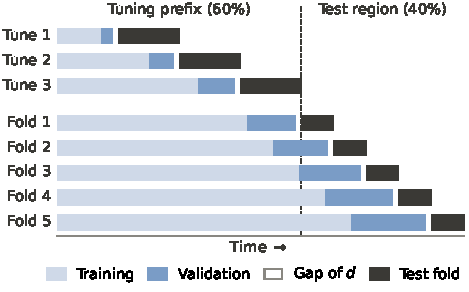
\includegraphics[width=\columnwidth]{cv_diagram}
\caption{Partitioning of a Series for Tuning and Final Evaluation}
\label{fig:cv}
\end{figure}

The final 20\% of each training set served as the validation set for
early stopping.
Each fold was standardised with the mean and the standard deviation of
the training set of the fold alone.
The test data therefore played no part in the scaling of the training
data.

\subsection{Hyperparameter Selection}

Each architecture received a separate search on each series.
A shared setting would favour whichever architecture the setting
happened to suit.
The Optuna library searched with the tree-structured Parzen
estimator~\cite{akiba2019}.
Each search evaluated 20 candidates.
Each candidate was scored by the mean Theil U statistic over three
expanding-window folds within the tuning prefix.
The upper rows of Figure~\ref{fig:cv} show the three tuning folds.
The tuning prefix was limited to the most recent 4000 observations.
The limit affected only the electricity series.
The electricity search used 4000 hours from May to October 2017.
The final runs used the year from August 2017 to August 2018.
The test region of the final runs began in March 2018.
Every tuning observation therefore preceded the test region.

The search covered four hyperparameters.
The number of hidden neurons was drawn from
$J \in \{2, 4, 8, 12, 16, 24, 32, 48, 64\}$.
The learning rate was drawn from $\eta \in [10^{-3}, 3 \times 10^{-2}]$
on a logarithmic scale.
The weight decay coefficient was drawn from
$\lambda \in \{0, 10^{-5}, 10^{-4}, 10^{-3}\}$.
The window length $d$ was the most series-specific choice.
The candidate windows were built around the known periods of each
series.
The Mackey-Glass windows $d \in \{10, 17, 25, 40\}$ bracket the delay
of 17.
The electricity windows $d \in \{24, 48, 72\}$ span one to three days.
A weekly window of 168 hours would require BPTT over 168 time steps.
The weekly window was excluded to avoid vanishing
gradients~\cite{bengio1994}.
The page views windows $d \in \{7, 14, 30, 60\}$ span one week to two
months.
The temperature windows $d \in \{7, 14, 30, 60, 90, 120\}$ extend to
four months.
The S\&P~500 windows $d \in \{5, 10, 20, 40\}$ span one to eight
trading weeks.
Each candidate trained for at most 60 epochs with a patience of eight.
Table~\ref{tab:tuning} lists the selected hyperparameters.

\begin{table}[t]
\centering
\caption{Selected Hyperparameters and Number of Weights}
\label{tab:tuning}
\footnotesize
\setlength{\tabcolsep}{4pt}
\begin{tabular}{@{}llrrrrr@{}}
\toprule
Series & Network & $d$ & $J$ & $\eta$ & $\lambda$ & Weights \\
\midrule
Mackey-Glass & Elman & 17 & 12 & 0.0264 & 0 & 181 \\
 & Jordan & 10 & 16 & 0.0256 & $10^{-4}$ & 65 \\
 & Multi-recurrent & 17 & 12 & 0.0289 & $10^{-5}$ & 661 \\
\midrule
Electricity & Elman & 72 & 48 & 0.0048 & 0 & 2449 \\
 & Jordan & 48 & 64 & 0.0170 & $10^{-3}$ & 257 \\
 & Multi-recurrent & 24 & 32 & 0.0061 & 0 & 4321 \\
\midrule
Page views & Elman & 14 & 16 & 0.0153 & $10^{-5}$ & 305 \\
 & Jordan & 30 & 32 & 0.0214 & $10^{-5}$ & 129 \\
 & Multi-recurrent & 14 & 16 & 0.0273 & 0 & 1137 \\
\midrule
Temperature & Elman & 30 & 32 & 0.0014 & $10^{-3}$ & 1121 \\
 & Jordan & 30 & 12 & 0.0022 & 0 & 49 \\
 & Multi-recurrent & 60 & 32 & 0.0035 & $10^{-4}$ & 4321 \\
\midrule
S\&P 500 & Elman & 20 & 4 & 0.0048 & $10^{-3}$ & 29 \\
 & Jordan & 5 & 16 & 0.0011 & $10^{-4}$ & 65 \\
 & Multi-recurrent & 5 & 24 & 0.0011 & $10^{-3}$ & 2473 \\
\bottomrule
\end{tabular}
\end{table}


\subsection{Training}

The final runs allowed longer training than the hyperparameter search.
Each network minimised the mean squared error with the Adam
optimiser~\cite{kingma2015}.
Mini-batches held 128 patterns.
The gradient norm was clipped at five~\cite{pascanu2013}.
Training ran for at most 200 epochs with a patience of 15.
Each architecture was trained with five different random seeds on each
of the five test folds.
Each combination of series and architecture thus produced 25 networks.
All architectures shared the same folds and the same seeds.
Differences in accuracy therefore reflect the architectures rather than
the data seen in training.

\subsection{Performance Measures}

Let $q$ denote the number of forecasts in a test fold.
The root mean squared error (RMSE) of the forecasts is
\begin{equation}
r = \sqrt{\frac{1}{q}\sum_{t} \left(x_t - \hat{x}_t\right)^2}.
\label{eq:rmse}
\end{equation}
The RMSE carries the units of the series.
An RMSE of 100 megawatts alone says little about the quality of an
electricity forecast.
A benchmark supplies the missing reference.
The persistence forecast $\hat{x}_{t+1} = x_t$ repeats the last
observation.
Let $\tilde{r}$ denote the RMSE of persistence.
The Theil U statistic $u = r / \tilde{r}$ divides the RMSE of a model by
the RMSE of persistence~\cite{theil1966}.
A value below one means the model improves on persistence.
A value of one means the model adds nothing to the last observation.
The Theil U statistic is free of units and therefore served as the
primary measure across all five series.

\subsection{Lag Study}

The fourth and fifth research questions look inside the trained
networks.
The lag $l$ of a forecast $\hat{x}_{t+1}$ refers to the observation
$x_{t+1-l}$.
Lag one is thus the most recent observation.

The first stage measured how strongly each forecast responds to each
lag.
Output sensitivity analysis measures the response through the
derivative of the output with respect to each input~\cite{engelbrecht1995}.
The sensitivity of the forecast to lag $l$ is
\begin{equation}
S_l = \frac{1}{P}\sum_{p=1}^{P}
\left| \frac{\partial o_{1,p}}{\partial x_{t+1-l,p}} \right|,
\label{eq:sensitivity}
\end{equation}
where $P$ is the number of patterns.
The symbol $x_{t+1-l,p}$ denotes the observation at lag $l$ in pattern
$p$.
Each sensitivity was divided by the sum over all lags in the window.
The resulting share gives the fraction of the total sensitivity
attributed to each lag.
The first stage used only the tuning prefix.
The networks trained on the first 80\% of the prefix.
The shares were measured on the remaining 20\% and averaged over five
seeds.

The second stage tested whether direct access to a single lag $L$
improves the forecast.
The lag $L$ was fixed in advance by the process that generated each
series.
Mackey-Glass used the delay $L = 17$.
Electricity used the daily cycle $L = 24$.
Page views and temperature used the annual cycle $L = 365$.
The S\&P~500 series used $L = 5$ trading days as a control.
A gain on the control would indicate an artefact of the procedure.

A second input channel supplied the standardised value of lag $L$ at
the final time step of each window.
The channel held zero at every earlier time step.
The value of lag $L$ therefore reached the hidden layer directly.
The effect of the shortcut depends on the position of the lag relative
to the window.
A lag inside the window already reaches the network at an earlier time
step.
The value then passes through $L-1$ recurrent steps before the forecast
is made.
The contribution of the value can fade with each step.
The shortcut delivers the value before the contribution fades.
A lag of 365 days lies outside every window.
The tuned window of the JRNN on Mackey-Glass also excludes lag 17.
The shortcut then supplies an observation the network would otherwise
never receive.
A gain for a lag outside the window mixes the effect of memory with the
effect of additional information.
Missing lag values at the start of a series were set to the training
mean.
The training mean equals zero after standardisation.
All other settings matched the final runs.
Every shortcut network therefore formed a pair with a network from the
final runs.

A data-driven choice of $L$ was also considered.
A rule specified in advance selected the lag with the largest share
above the trend of the neighbouring lags.
The rule mostly selected lag two or lag three.
The rule also selected a lag on the control series, where no dependence
was expected.
The rule was therefore rejected before any shortcut network was trained.

\subsection{Analysis Procedure}

The analysis procedure matched each research question to a statistical
test.
Each combination of fold and seed formed one block.
Each series therefore contributed 25 blocks.
The Theil U statistics of all architectures were paired within each
block.
All tests used a significance level of 0.05.
The Friedman test compares several paired samples through ranks within
each block~\cite{friedman1937}.
The Wilcoxon signed-rank test compares two paired
samples~\cite{wilcoxon1945}.
The Holm procedure adjusts the $p$-values of a family of
tests~\cite{holm1979}.

The first question asks whether the architectures differ.
A Friedman test compared the three architectures on each series.
A rejection was followed by two-sided Wilcoxon tests on the three pairs
with the Holm adjustment.
Across series the architectures were ranked by mean Theil U statistic.
A Friedman test on the average ranks compared the architectures across
the five series~\cite{demsar2006}.
The Nemenyi critical difference identified significantly different
average ranks~\cite{demsar2006}.

The second question asks when the architectures differ.
One-sided Wilcoxon tests examined whether each architecture improved on
persistence with a Theil U statistic below one.
The differences between the architectures were then compared along the
predictability range of the series.
The third question weighs accuracy against weights.
The pairwise comparison of the ERNN and the MRNN was read together with
the number of weights in Table~\ref{tab:tuning}.

The fourth question was answered by the sensitivity shares at lag one
and at lag $L$.
The fifth question was answered by two-sided Wilcoxon tests between each
shortcut network and the paired network from the final runs.
The Holm procedure adjusted the 15 resulting $p$-values.

Two properties of the design limit the interpretation of the tests.
The five seeds of a fold share the same training and test data.
The 25 blocks of a series are therefore not independent.
The reported $p$-values are optimistic as a result.
A robustness check addressed the dependence.
The check averaged the Theil U statistics over the seeds of each fold.
Five values per architecture then remained on each series.
The check counted the folds where each difference kept the same
direction.
A difference consistent on all five folds does not rest on the
dependence between seeds.
The second property concerns the window lengths.
Different window lengths gave the architectures slightly different test
targets.

% ======================================================================
\section{Results and Discussion}
\label{sec:results}
The results follow the order of the research questions.
The selected hyperparameters come first because the hyperparameters
shape every later comparison.
The effect of the feedback source and the role of predictability
follow.
The comparison of the MRNN with the ERNN precedes the two stages of the
lag study.
The forecasts themselves and a discussion of the limitations close the
section.

\begin{figure*}[t]
\centering
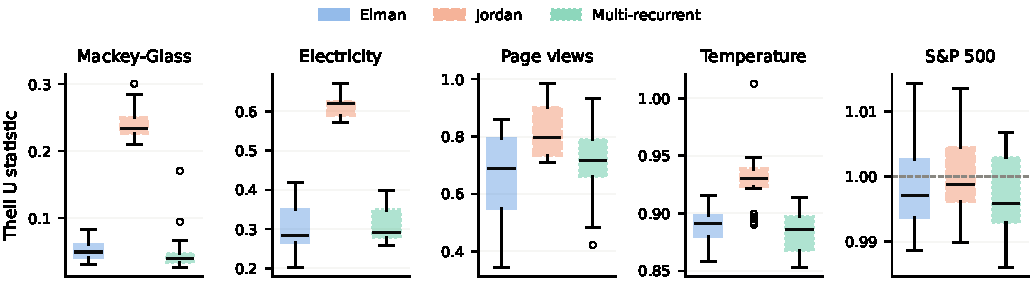
\includegraphics[width=\textwidth]{theil_boxplots}
\caption{Distribution of the Theil U Statistic Over the 25 Blocks of
Each Series}
\label{fig:boxplots}
\end{figure*}

\subsection{Hyperparameter Selection}

Table~\ref{tab:tuning} reveals three patterns in the selected
hyperparameters.
The first pattern concerns the JRNN.
The search gave the JRNN more hidden neurons than the ERNN on four of
the five series.
On electricity the JRNN reached the largest candidate of $J = 64$.
A wider range could have benefited the JRNN on electricity.
The JRNN still had fewer weights than the ERNN on four of the five
series.
Additional hidden neurons cannot enlarge the single fed-back value of
the JRNN.

The second pattern concerns the size of the networks.
The search adapted the capacity of the ERNN to the structure of each
series.
The ERNN received the most hidden neurons on electricity with $J = 48$.
Electricity combines daily and weekly cycles with a seasonal swing.
The ERNN on the S\&P~500 series received only four hidden neurons with
the strongest weight decay.
A random walk offers nothing for additional weights to learn.
The MRNN had about four times the weights of the ERNN on three series.
The ratio fell to 1.8 on electricity and reached 85 on the S\&P~500
series.

The third pattern concerns the windows.
The ERNN and the MRNN selected the window $d = 17$ on Mackey-Glass.
The window matched the delay $\tau = 17$ exactly.
The JRNN selected the shorter window of ten observations.
The single fed-back value of the JRNN explains the choice.
Observations early in a long window barely reach the forecast of a JRNN.
A longer window adds BPTT steps without adding usable information.
The short window also excluded the delay from the JRNN.


\subsection{Effect of the Feedback Source}

Table~\ref{tab:theil} lists the mean Theil U statistic of each
architecture on each series.
The Friedman test rejected equal performance on every series with
$p \leq 0.012$.
The JRNN had the highest mean Theil U statistic on every series.
The pairwise tests found the JRNN significantly less accurate than both
other architectures on the four structured series with adjusted
$p \leq 0.003$.
The difference held on all five folds for three of the four series.
Page views showed the same direction on four of the five folds.
The size of the gap varied widely.
On Mackey-Glass the JRNN reached a Theil U statistic of 0.240 against
0.051 for the ERNN.
The error of the JRNN was thus 4.7 times the error of the ERNN.


\begin{table}[t]
\centering
\caption{Mean and Standard Deviation of the Theil U Statistic}
\label{tab:theil}
\footnotesize
\begin{tabular}{@{}lccc@{}}
\toprule
Dataset & Elman & Jordan & Multi-recurrent \\
\midrule
Mackey-Glass & 0.0511 $\pm$ 0.0146 & 0.2401 $\pm$ 0.0225 & \textbf{0.0479 $\pm$ 0.0291} \\
Electricity & \textbf{0.3037 $\pm$ 0.0599} & 0.6105 $\pm$ 0.0254 & 0.3117 $\pm$ 0.0444 \\
Page views & \textbf{0.6629 $\pm$ 0.1582} & 0.8231 $\pm$ 0.1009 & 0.7170 $\pm$ 0.1205 \\
Temperature & 0.8884 $\pm$ 0.0175 & 0.9293 $\pm$ 0.0247 & \textbf{0.8845 $\pm$ 0.0189} \\
S\&P 500 & 0.9981 $\pm$ 0.0063 & 0.9997 $\pm$ 0.0059 & \textbf{0.9968 $\pm$ 0.0061} \\
\bottomrule
\end{tabular}
\end{table}


The ERNN and the MRNN did not differ significantly on any series.
The adjusted $p$-values of the comparison lay between 0.12 and 0.34.
On the S\&P~500 series only the MRNN differed significantly from the
JRNN.
The difference amounted to 0.003 in the Theil U statistic.
Across the five series the MRNN achieved the best average rank of 1.4.
The ERNN followed with an average rank of 1.6.
The JRNN ranked last on every series.
The Friedman test on the average ranks rejected equal performance with
$p = 0.022$.
The Nemenyi critical difference of 1.48 separated only the JRNN from
the MRNN.
The gap of 1.4 between the JRNN and the ERNN fell just short of the
critical difference.
Five series offer little power for the Nemenyi test.

The source of the fed-back values therefore affected accuracy.
Feedback of the output alone produced consistently less accurate
forecasts than feedback of the hidden layer.

\begin{figure*}[t]
\centering
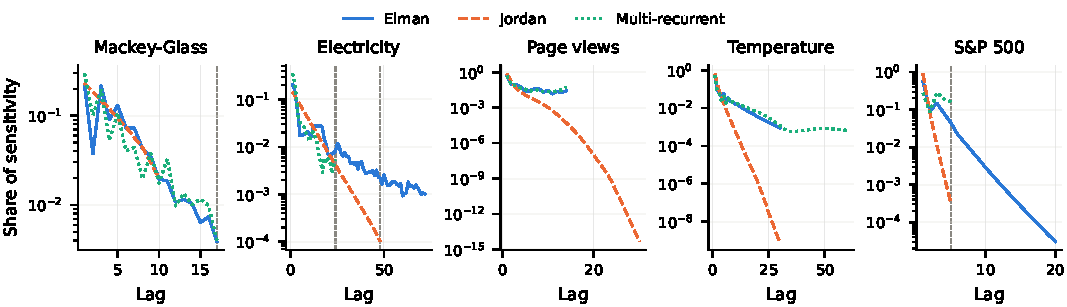
\includegraphics[width=\textwidth]{sensitivity_profiles}
\caption{Share of Sensitivity per Lag Averaged Over Five Seeds}
\label{fig:sensitivity}
\end{figure*}

\subsection{Dependence on Predictability}

Figure~\ref{fig:boxplots} shows the distribution of the Theil U
statistic over the 25 blocks of each series.
The Theil U statistic of the ERNN rose from 0.051 on Mackey-Glass to
0.998 on the S\&P~500 series.
The order of the series by Theil U statistic matched the range of
predictability set out in the introduction.
Every architecture improved significantly on persistence on the four
structured series.
The improvement held on all five folds in every case.


The relative gap between the architectures shrank as predictability
fell.
The ratio of the Theil U statistic of the JRNN to the Theil U statistic
of the ERNN measures the relative gap.
The ratio fell from 4.7 on Mackey-Glass to 2.0 on electricity.
The ratio fell further to 1.24 on page views and 1.05 on temperature.
On the S\&P~500 series the ratio reached 1.00.
The difference between the Theil U statistics behaved differently.
The largest difference of 0.307 occurred on electricity.
On Mackey-Glass both architectures lay close to zero.
A large relative gap therefore produced only a small difference.

On the S\&P~500 series only the MRNN improved significantly on
persistence with an adjusted $p = 0.028$.
The improvement held on only three of the five folds.
The networks on the S\&P~500 series behaved close to persistence.
The standard deviation of the forecast returns amounted to between 3\%
and 9\% of the standard deviation of the actual returns.
The mean forecast return of 0.00035 to 0.00062 per day was of the same
size as the average daily drift of about 0.0004 in the training data.
A drift-only forecast multiplies the last price by the exponential of
the mean training return.
The drift-only forecast achieved a mean Theil U statistic of 0.998.
The mean Theil U statistic of every network lay within 0.0015 of the
drift-only forecast.
The small improvement on persistence therefore reflects the historical
upward drift of the index rather than learned structure.



\subsection{Memory Banks versus Weights}

The third research question weighs the accuracy of the MRNN against the
cost of the memory banks.
The pairwise tests found no significant difference between the ERNN and
the MRNN on any series.
The folds nevertheless reveal a small consistent pattern in favour of
the MRNN.
On every series except electricity and page views the MRNN had the
lower mean Theil U statistic.
The MRNN was also more accurate on four of the five folds of each of
these series.
The largest of these leads amounted to only 0.004.

The ERNN led on the remaining two series.
The lead of the ERNN on page views reached 0.054 but held on only three
of the five folds.
The wide spread of the page views results produced the large but
inconsistent lead.
Neither architecture therefore held a lead that was both large and
consistent.

The memory banks came at a considerable cost.
The MRNN had about four times the weights of the ERNN on most series.
A consistent gain of at most 0.004 in the Theil U statistic has no
practical value at such a cost.
The memory banks therefore did not justify the additional weights.

\subsection{Sensitivity to Past Observations}

Figure~\ref{fig:sensitivity} shows the sensitivity profiles of the three
architectures.
A dashed line marks the delay of 17 on Mackey-Glass.
On electricity dashed lines mark the daily lags of 24 and 48 hours.
A dashed line also marks lag five on the S\&P~500 control.
The annual lag lies outside every window on page views and temperature.
Lag one dominated every profile.
The share of lag one ranged from 0.14 to 0.35 on Mackey-Glass and
electricity.
On the S\&P~500 series the JRNN placed a share of 0.90 on lag one.
The JRNN on the S\&P~500 series thus behaved almost as a persistence
forecast.

Sensitivity fades with the lag in every recurrent network.
An earlier observation passes through more recurrent steps before the
forecast.
A small share at a distant lag therefore does not by itself show that
the lag carries little information.
The comparison of the architectures rests on the rate of decay instead.
On electricity the sensitivity of the JRNN fell exponentially with the
lag.
The same decay appeared on page views and temperature.
The profile of the JRNN therefore appears as a straight line on the
logarithmic axis.
On temperature the share of the JRNN fell below $10^{-8}$ by lag 30.
On page views the share fell below $10^{-12}$ by lag 30.
The profiles of the ERNN and the MRNN on the same series stayed above
$10^{-4}$.
On Mackey-Glass the short windows kept all three profiles close
together.
On the S\&P~500 series the profile of the ERNN also fell exponentially.
A random walk offers no distant information worth keeping.
The steep decay of the JRNN matches the single fed-back value.
Information from an early observation reaches the forecast of a JRNN
only through a chain of single fed-back values.
Each link of the chain scales the contribution by a similar factor.

A network that relied on a known lag would show a rise above the fading
trend at that lag.
The residual rule of the lag study measured such a rise at every lag.
The rule compared the logarithmic share of each lag with a straight line
fitted to the three neighbouring lags on either side.
A lag counted as prominent only above 1.65 times the local trend.
On Mackey-Glass the rule selected lag three instead of the delay of 17.
On electricity the rule selected lag 25 for the ERNN.
Lag 25 holds the load one day before the latest observation.
The share of lag 25 lay 1.5 times above the local trend.
The rise fell short of the threshold for prominence.
The ERNN thus showed a weak response to the daily cycle.
The delay on Mackey-Glass drew no such response.
The ERNN and the MRNN placed a share of 0.004 on lag 17.
The same networks had selected windows that include lag 17 exactly.
The delay thus shaped the choice of window without drawing a large
direct response.

\subsection{Direct Access to a Known Lag}

Table~\ref{tab:shortcut} lists the Theil U statistic of each network
with and without the shortcut.
The shortcut reduced the Theil U statistic significantly in four of the
15 comparisons.
Three of the four significant reductions involved the JRNN.
Every significant reduction held on all five folds.

\begin{table}[t]
\centering
\caption{Theil U Statistic With and Without the Shortcut}
\label{tab:shortcut}
\footnotesize
\setlength{\tabcolsep}{3pt}
\begin{tabular}{@{}llrrcccc@{}}
\toprule
Series & Network & $L$ & $d$ & Final & Shortcut & Adj.\ $p$ & Folds \\
\midrule
Mackey-Glass & Elman  & 17 & 17 & 0.0511 & 0.0434 & 0.354 & 4 \\
             & Jordan & 17 & 10 & 0.2401 & 0.0733 & $<0.001$ & 5 \\
             & Multi  & 17 & 17 & 0.0479 & 0.0371 & 0.089 & 4 \\
\midrule
Electricity  & Elman  & 24 & 72 & 0.3037 & 0.3031 & 1.000 & 3 \\
             & Jordan & 24 & 48 & 0.6105 & 0.5938 & 0.001 & 5 \\
             & Multi  & 24 & 24 & 0.3117 & 0.3141 & 1.000 & 1 \\
\midrule
Page views   & Elman  & 365 & 14 & 0.6629 & 0.6898 & 1.000 & 1 \\
             & Jordan & 365 & 30 & 0.8231 & 0.8141 & 1.000 & 3 \\
             & Multi  & 365 & 14 & 0.7170 & 0.7228 & 1.000 & 2 \\
\midrule
Temperature  & Elman  & 365 & 30 & 0.8884 & 0.8863 & 0.027 & 5 \\
             & Jordan & 365 & 30 & 0.9293 & 0.9135 & 0.001 & 5 \\
             & Multi  & 365 & 60 & 0.8845 & 0.8844 & 1.000 & 4 \\
\midrule
S\&P~500     & Elman  & 5 & 20 & 0.9981 & 1.0013 & 0.115 & 2 \\
             & Jordan & 5 & 5  & 0.9997 & 1.0008 & 1.000 & 2 \\
             & Multi  & 5 & 5  & 0.9968 & 0.9978 & 1.000 & 1 \\
\bottomrule
\end{tabular}
\end{table}

The largest gain occurred for the JRNN on Mackey-Glass.
The Theil U statistic fell from 0.240 to 0.073.
The shortcut closed 88\% of the gap between the JRNN and the ERNN.
The tuned window of the JRNN excluded lag 17.
The shortcut therefore supplied an observation the JRNN never received.
The gain on Mackey-Glass reflects the value of the delayed observation
rather than an improvement in memory.
The ERNN and the MRNN on Mackey-Glass improved on four of the five
folds.
The improvements did not remain significant after the Holm adjustment.

Electricity provides the cleaner test.
Lag 24 lies inside the window of every architecture.
The shortcut reduced the Theil U statistic of the JRNN from 0.611 to
0.594.
The reduction held on all five folds.
The ERNN and the MRNN showed no significant change.
The ERNN already showed a weak response near the daily lag in the first
stage.
The shortcut thus helped only the architecture with the fastest-fading
memory.

On temperature the shortcut reduced the Theil U statistic of the JRNN
from 0.929 to 0.914.
The ERNN improved by only 0.002.
The annual lag lies outside every window on temperature.
The temperature gains therefore reflect additional information alone.
The temperature one year earlier indicates the typical level for the
time of year.
A window of 30 to 60 days cannot supply the level directly.
The JRNN gained more than the ERNN.
A network that uses little of the window benefits most from an extra
reference value.
The annual lag brought no significant change on page views.
The tournament moves by several days from year to year.
The view count 365 days earlier can therefore miss the onset of the
spike.

The control showed no significant change for any architecture.
The shortcut therefore improved accuracy only where a real dependence
existed.
The MRNN placed a share of 0.16 on lag five of the S\&P~500 series.
The shortcut at lag five still brought no gain.
A large sensitivity share therefore does not identify a useful lag.

\begin{figure*}[t]
\centering
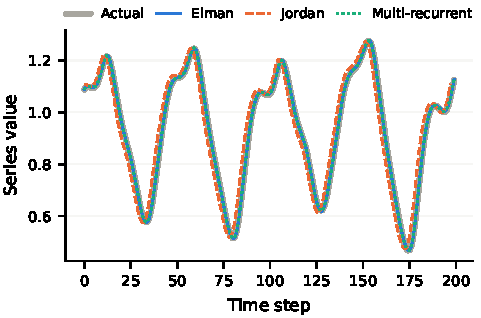
\includegraphics[width=\columnwidth]{forecast_mackey_glass}\hfill
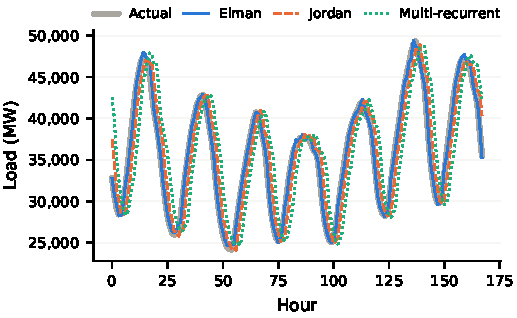
\includegraphics[width=\columnwidth]{forecast_electricity}\\[4pt]
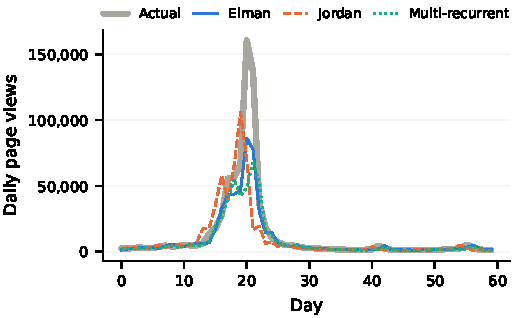
\includegraphics[width=\columnwidth]{forecast_pageviews}\hfill
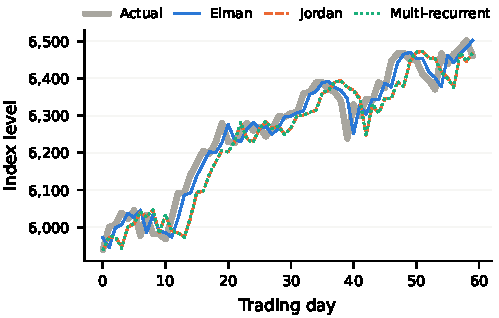
\includegraphics[width=\columnwidth]{forecast_sp500}
\caption{Forecasts on the Final Test Fold of Four Series}
\label{fig:forecasts}
\end{figure*}

\subsection{Forecast Behaviour}

Figure~\ref{fig:forecasts} shows the forecasts of the first seed on the
final test fold of four series.
The panels show Mackey-Glass and electricity in the top row.
The panels show page views and the S\&P~500 series in the bottom row.
A forecast shifted to the right of the actual series reproduces a
change only after the change has occurred.
A forecast shifted to the left reproduces a change before the change
occurs.
The persistence forecast is the actual series shifted one step to the
right.

The ERNN and the MRNN on Mackey-Glass lay on top of the actual series.
The JRNN ran about one step ahead of the actual series throughout the
fold.
The dynamics of Mackey-Glass depend on the value 17 steps earlier.
The window of the JRNN excluded the delayed value.
A forecast that runs ahead fits a network that extrapolates the recent
trend of the series too far. 

On electricity every architecture reproduced the daily cycle.
The ERNN followed the actual series closely at every hour.
The JRNN trailed the actual series by about one hour throughout the
daily cycle.
The steep daily ramps turn a lag of one hour into a large error.
The lag explains much of the gap between the Theil U statistic of 0.61
for the JRNN and 0.30 for the ERNN.

On page views the views rose for about a week before the peak.
Every architecture followed the rise but undershot the peak of about
160\,000 views.
The ERNN reached about 87\,000 views on the day of the peak.
The JRNN forecast values above the actual views in the days before the
peak.
The JRNN peaked one day early.
The early rise matches the extrapolation of the recent trend seen on
Mackey-Glass.

On the S\&P~500 series the ERNN traced the actual series shifted by one
day.
The shift is the signature of a forecast close to persistence.
The JRNN and the MRNN lagged further and smoothed the daily moves.

The temperature forecasts are not shown for space.
All architectures followed the slow seasonal rise of the temperature
over the final fold.
The forecasts moved with the day-to-day swings but by a smaller amount.
The forecasts reached neither the cold troughs nor the warm peaks.
Sharp changes reappeared in the forecasts about one day late.

\subsection{Discussion}

The results identify the fed-back values as the bottleneck of the JRNN.
The search gave the JRNN more hidden neurons than the ERNN on four
series.
The additional neurons did not close the gap.
The sensitivity profiles showed the memory of the JRNN fading
exponentially.
The shortcut repaired part of the deficit by delivering a single past
value.
The original formulation of Jordan gave each state neuron a
self-connection~\cite{jordan1986}.
A self-connection keeps a slowly fading copy of earlier outputs.
The self-connections target the observed weakness directly.

The MRNN presents the opposite case.
The memory banks added weights without adding useful information.
The input window already supplied the recent history.
The context layer of the ERNN apparently carried the remaining history.
Richer feedback therefore brought no benefit beyond the feedback of the
hidden layer.

Three limitations qualify the results.
The first limitation concerns the hyperparameter search.
The search capped training at 60 epochs.
The median best epoch of the final Mackey-Glass networks ranged from 68
for the MRNN to 97 for the JRNN.
The search on Mackey-Glass could therefore have favoured settings that
learn quickly.
The second limitation concerns the MRNN.
The decay rates of the memory banks were fixed rather than tuned.
Other decay rates could suit series with long cycles better.
The final limitation concerns the S\&P~500 series.
The logarithmic returns remove the random walk but not the changes in
volatility between market regimes.
On the third test fold every architecture performed worse than
persistence.
The drift-only forecast also performed worse than persistence on the
same fold.

\section{Conclusions}
\label{sec:conclusions}
The study compared three simple recurrent architectures on five
univariate series.
The Elman recurrent neural network (ERNN) fed back the hidden layer.
The Jordan recurrent neural network (JRNN) fed back the output.
The multi-recurrent neural network (MRNN) fed back both through memory
banks.

The source of the fed-back values affected accuracy.
The JRNN was significantly less accurate than the ERNN and the MRNN on
all four structured series.
The error of the JRNN reached 4.7 times the error of the ERNN on
Mackey-Glass.
The relative gap shrank as the predictability of the series fell.
On the S\&P~500 series every architecture stayed close to persistence
plus the historical drift.
The memory banks of the MRNN gained at most 0.004 in the Theil U
statistic over the ERNN.
The gain did not justify about four times the weights.

The lag study explained the weakness of the JRNN.
The sensitivity of the JRNN to past observations fell exponentially
with the lag.
The ERNN and the MRNN retained access to distant lags on the structured
series.
Direct access to a known lag helped mainly the JRNN.
On Mackey-Glass the shortcut reduced the Theil U statistic of the JRNN
from 0.240 to 0.073.
The single fed-back value of the JRNN therefore limited the memory of
the network.

Two directions for future work follow from the results.
The final jump to the peak of the page views series exceeded every
forecast.
An input that marks the dates of the tournament could supply the
missing information.
Jordan originally gave each state neuron a
self-connection~\cite{jordan1986}.
A self-connection keeps a fading copy of earlier outputs.
A comparison of the JRNN with and without self-connections would test
the explanation of the weakness directly.

The results suggest a limit on the value of memory.
A single fed-back value left the JRNN short of memory.
Beyond the memory of the ERNN additional feedback added weights without
adding accuracy.

\bibliographystyle{IEEEtranS}
\bibliography{refs}

\end{document}